\begin{figure}[H]
  \centering
  \begin{subfigure}[t]{.55\textwidth}
    \centering
    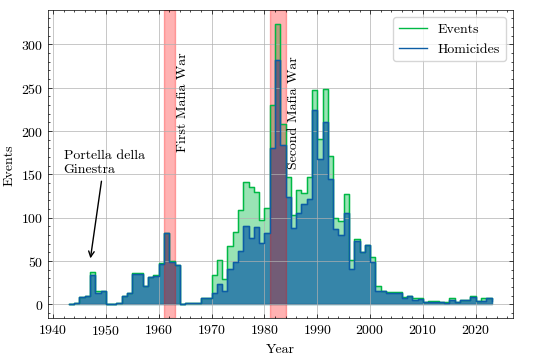
\includegraphics[width=\textwidth]{figures/omicidi.png}
    \caption{Monthly distribution of events in the dataset, with annotations highlighting significant periods. Each time, the number of violent events rises to a peak and then abruptly drops off.}
    \label{fig:omicidi}
  \end{subfigure}%
  \begin{subfigure}[t]{.36\textwidth}
    \centering
    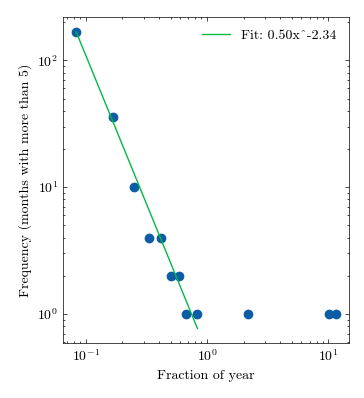
\includegraphics[width=\textwidth, trim={0 0.6cm 0 0},clip]{figures/intertimes.png}
    \caption{Log-log plot of inter-event times (with precision of months), only for months with more than 5 homicides. The distribution is a power-law.}
    \label{fig:intertimes}
  \end{subfigure}
  \caption{Examples of time analysis of the murders dataset.}
\end{figure}
